% sips -s format png your_pdf_file.pdf --out your_png_file.png

\documentclass[tikz,border=0mm]{standalone}

\usepackage{amsmath}
\usepackage{graphicx}
\usepackage[T1]{fontenc}
\renewcommand\familydefault{\sfdefault} 

\usetikzlibrary{arrows,shapes,calc,math,decorations.fractals,patterns,backgrounds,decorations.markings,decorations.pathmorphing}

\tikzset{point/.style={fill,circle,inner sep=1.5pt}}
\tikzset{vector/.style={-triangle 45, line width=1pt}}
\tikzset{dblarrow/.style={latex'-latex'}}
\tikzset{partial ellipse/.style args={#1:#2:#3}{insert path={+ (#1:#3) arc (#1:#2:#3)}}}
\tikzset{xaxis/.style={-stealth',red,line width=1pt}}
\tikzset{yaxis/.style={-stealth',green!80!black,line width=1pt}}
\tikzset{zaxis/.style={-stealth',blue,line width=1pt}}
\renewcommand{\vec}{\mathbf}


\begin{document}

% Logo
% \begin{tikzpicture}
%     \node {\includegraphics[width=5cm]{../Python_logo_and_wordmark.svg.png}};
%     \node at (0,-1) {\Huge \tt programming};
% \end{tikzpicture}

% Spyder window
% \begin{tikzpicture}
%     \node {\includegraphics{../1_Spyder.png}};
%     \draw [red,line width=4pt] (2,-13.2) rectangle ++(21.7,12.5);
%     \node [red] at ($(2,-13.2)!0.5!(23.7,-1)$) {\Huge \bf Console pane};
%     \draw [green,line width=4pt] (-23.5, -13.2) rectangle ++(25,25);
%     \node [green] at ($(-23.5,-13.2)!0.5!(1.5,11.8)$) {\Huge \bf Editor pane};
% \end{tikzpicture}

% Function
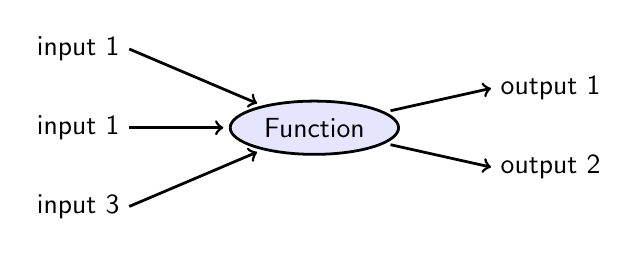
\begin{tikzpicture}
    \node [draw,fill=blue!10,ellipse,line width=1pt] (function) {Function};
    \node [left of=function,node distance=3cm] (input2) {input 1};
    \node [above of=input2] (input1) {input 1};
    \node [below of=input2] (input3) {input 3};
    \node [right of=function,node distance=3cm,yshift=0.5cm] (output1) {output 1};
    \node [right of=function,node distance=3cm,yshift=-0.5cm] (output2) {output 2};
    \draw [->,shorten >= 2pt,line width=1pt] (input1.east) to (function);
    \draw [->,shorten >= 2pt,line width=1pt] (input2) to (function);
    \draw [->,shorten >= 2pt,line width=1pt] (input3.east) to (function);
    \draw [->,shorten <= 2pt,line width=1pt] (function) to (output1.west);
    \draw [->,shorten <= 2pt,line width=1pt] (function) to (output2.west);
\end{tikzpicture}

\end{document}